\chapter{System Test}
\section{Calibration}\label{s:cals}
Calibration factor is obtained per cavity and in the vertical plane $y$ by measuring the position signal change as a function of the systematic cavity displacement. Two factors are used to obtain each calibration : the movers displacement vs voltage setting $C_m$ [$\mu$m/V] and the cavity response vs voltage setting $C_c$ [a.u./V]. Therefore the cavity calibration factor is $C_{bpm}=C_c/C_m$ [a.u./$\mu$m].\par
\subsection{Movers Calibration $C_m$}\label{s:calcm}
Previous to installation, the movers displacement vs Voltage setting was measured per BPM block. An interferometer with better than 1 nm resolution is used to measure the BPM vertical position as in Fig. (\ref{f:interfero}). As the head is located over the BPM, positive displacement implies negative change in the intereferometer lecture. Four cycles are shown in Fig. (\ref{f:fourcycles}), two descending and two rising, on the total dynamic range divided in 100 steps and 3 s between steps.\par
\begin{figure}[!htb]
\centering
\begin{subfigure}[b]{0.3\textwidth}
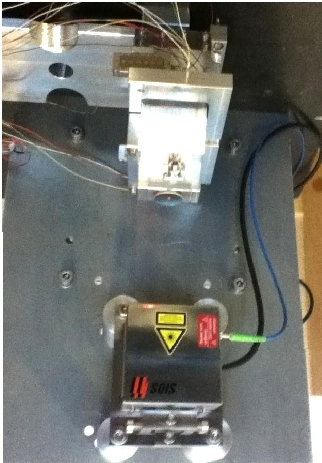
\includegraphics[scale=0.3,angle=180]{interfero.jpg}\caption{Picture of SIOS interferometer used to test the movers. Precision is better than 1 nm.}\label{f:interfero}
\end{subfigure}\hspace*{1cm}
\begin{subfigure}[b]{0.5\textwidth}
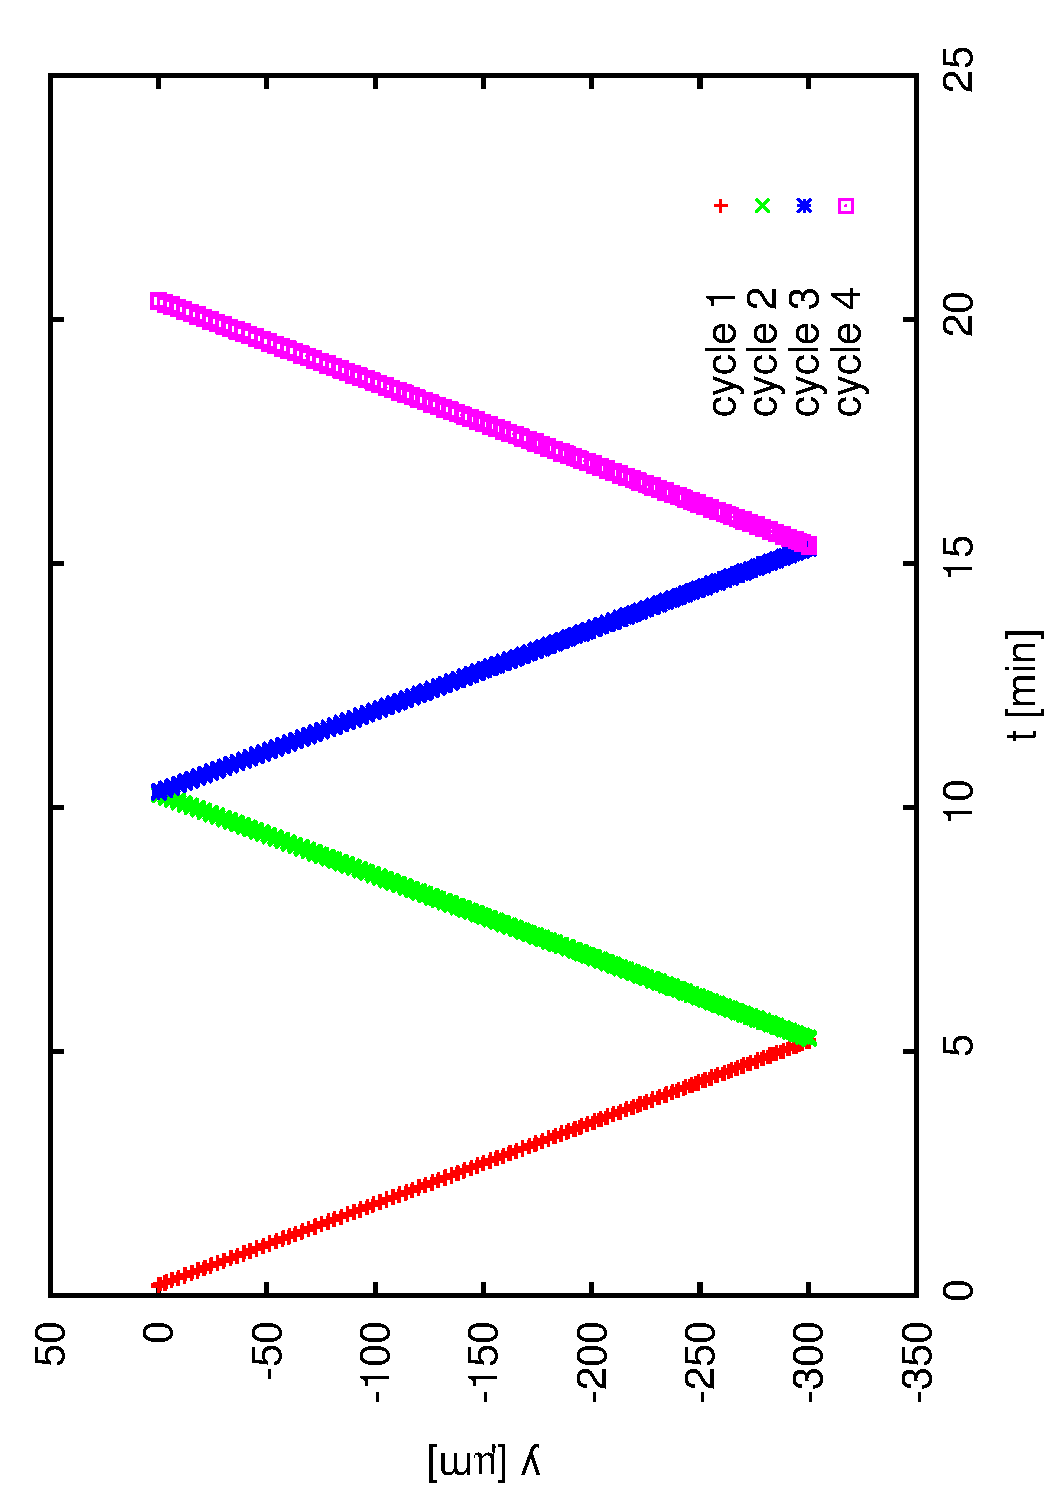
\includegraphics[scale=0.32,angle=-90]{image01.pdf}\caption{Four cycles are performed over the entire dynamic range of movers.}\label{f:fourcycles}
\end{subfigure}\caption{Movers calibration test setup for the vertical plane.}\label{f:cmtest}
\end{figure}
\subsubsection{Block AB movers, Cedrat}
Linearity was tested in the four cycles with feedback. Fig. (\ref{f:Cedratmsteps}) shows the mover step and Fig. (\ref{f:Cedratlinres}) shows the residuals from the linear fitting substraction on each cycle.\par
\begin{figure}[!htb]
 \centering\hspace*{-0.6cm}
\begin{subfigure}{0.4\textwidth}
 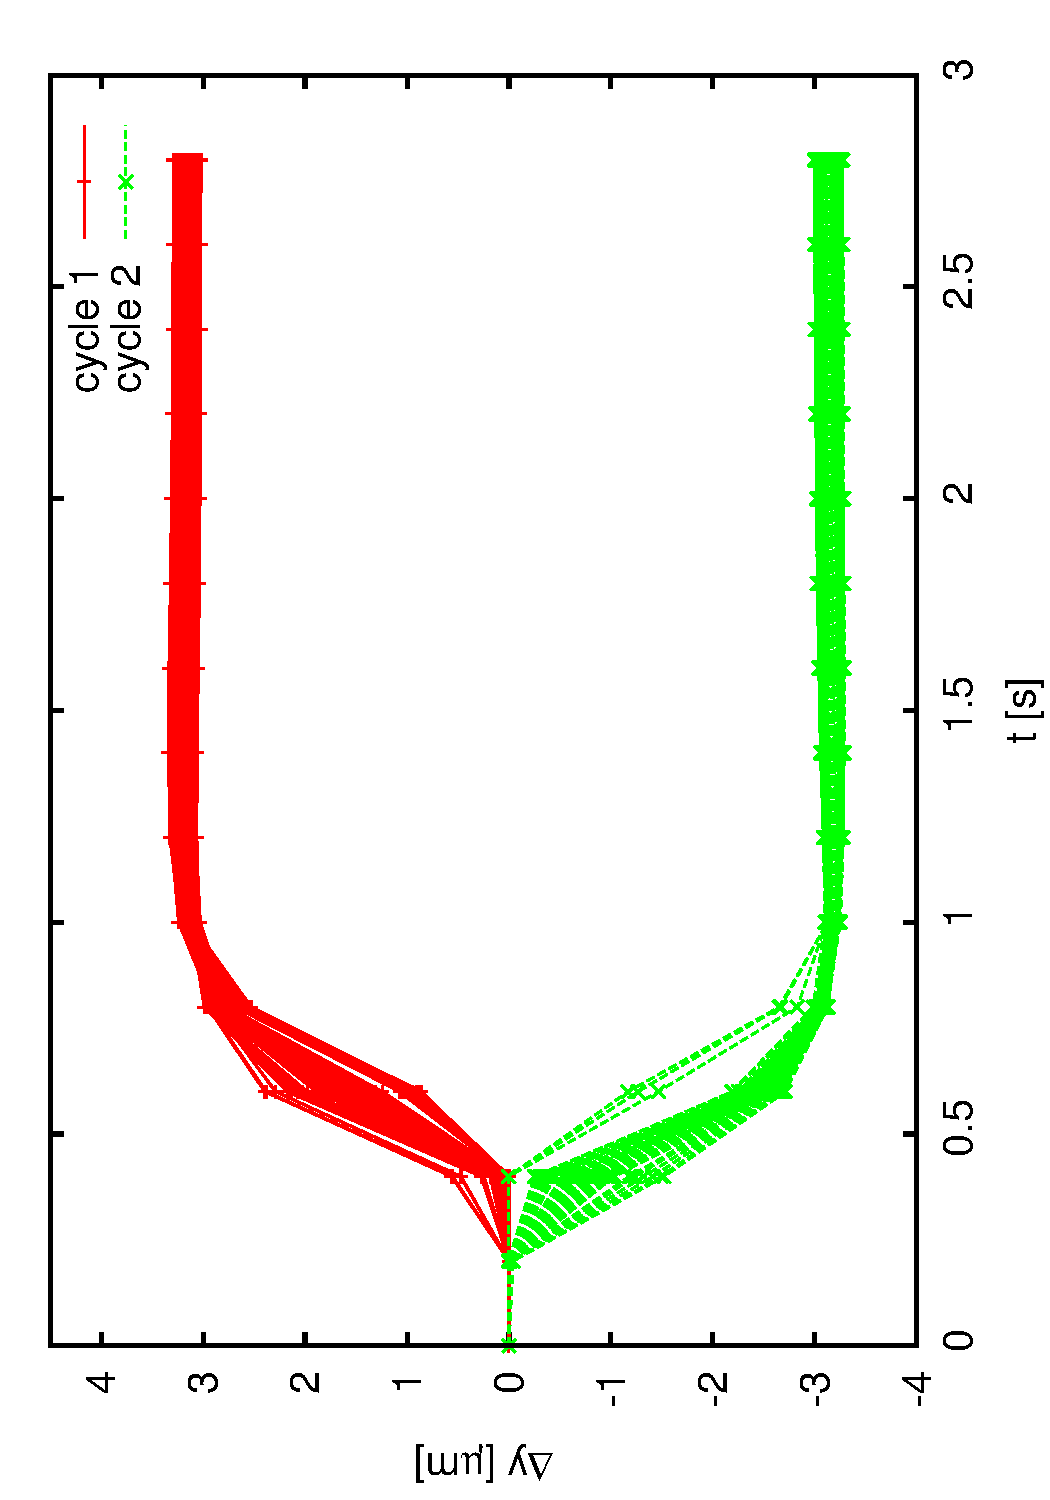
\includegraphics[angle=-90,scale=0.30]{image24.pdf}\caption{Settling speed with feedback for Cedrat movers.}\label{f:Cedratmsteps}
\end{subfigure}\hspace*{1.5cm}
\begin{subfigure}{0.4\textwidth}
 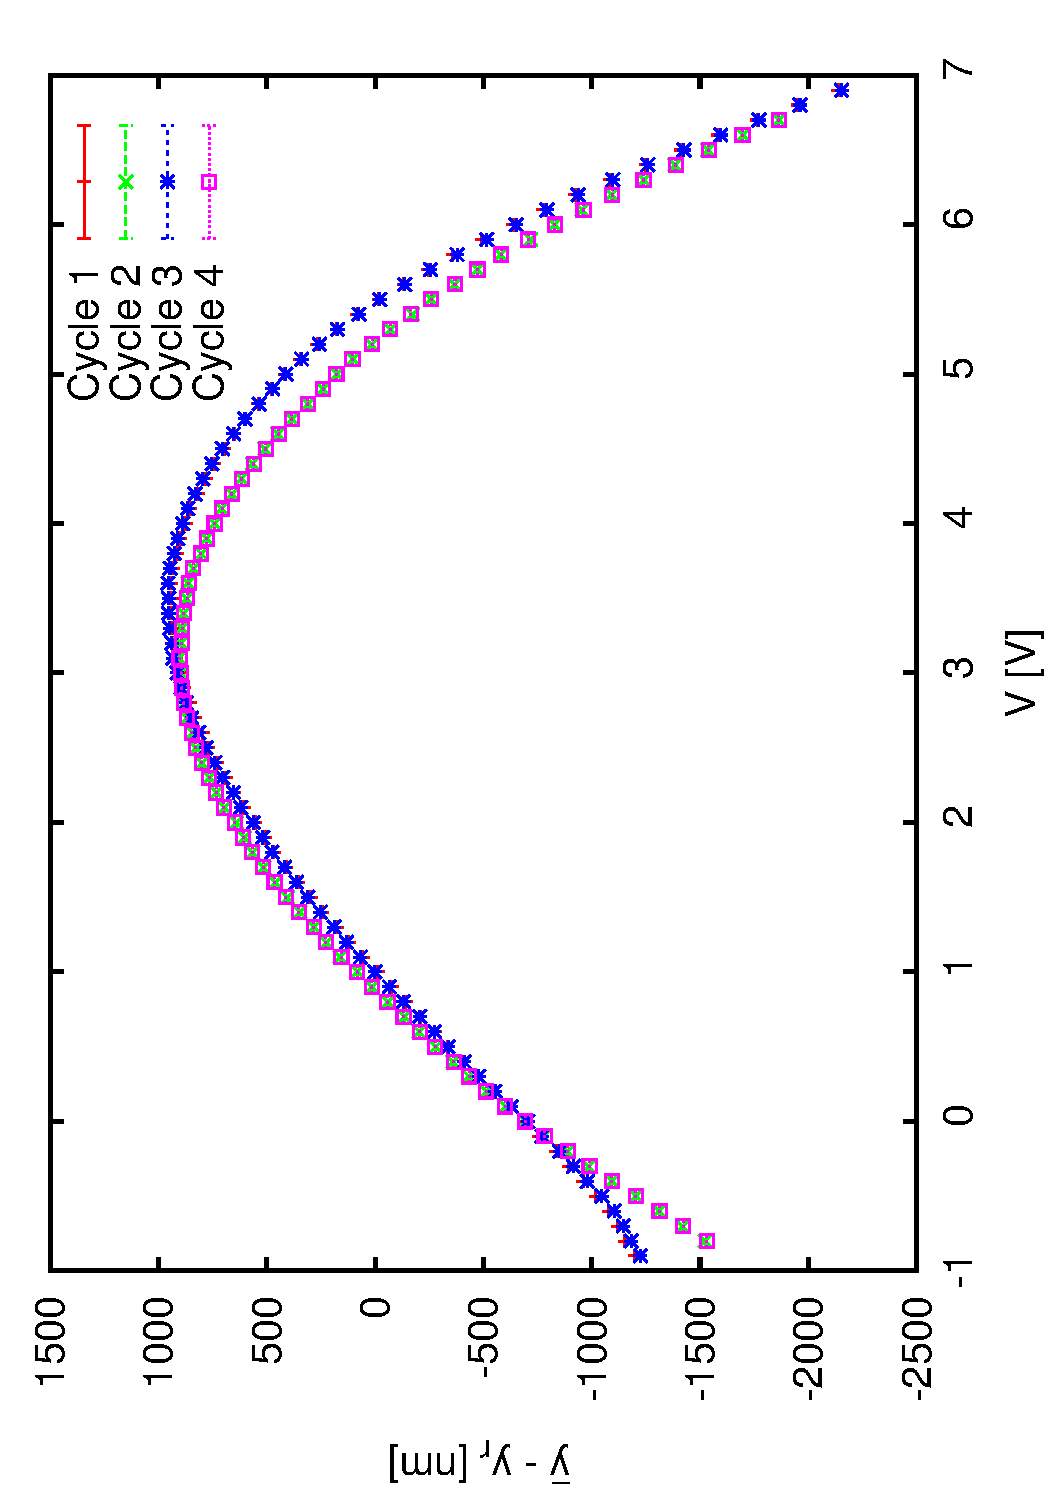
\includegraphics[angle=-90,scale=0.30]{image26e.pdf}\caption{Residual non-linearity (with fb), after substraction of linear fitting on cedrat movers.}\label{f:Cedratlinres}
\end{subfigure}\caption{Block AB movers, linearity test over four cycles.}\label{f:Cedratfeedback}
\end{figure}
The calibration mean from these 4 cycles is $C_{mAB} = (-31.015\pm12)\mu$m/V. This value is valid for ranges were the residual is constant, therefore, it is recommended to use the movers with voltage settings in the middle of the total dynamic range and scans over less than 1 V.\par
The step stability was tested by moving back and forth the voltage setting hundreds of times. Fig. (\ref{f:Cedratstepstab}) shows that 10 nm steps are observable and Fig. (\ref{f:Cedratstab}) shows 1.1 nm of stability on each setting.\par
\begin{figure}[!htb]
 \centering\hspace*{-0.6cm}
\begin{subfigure}{0.4\textwidth}
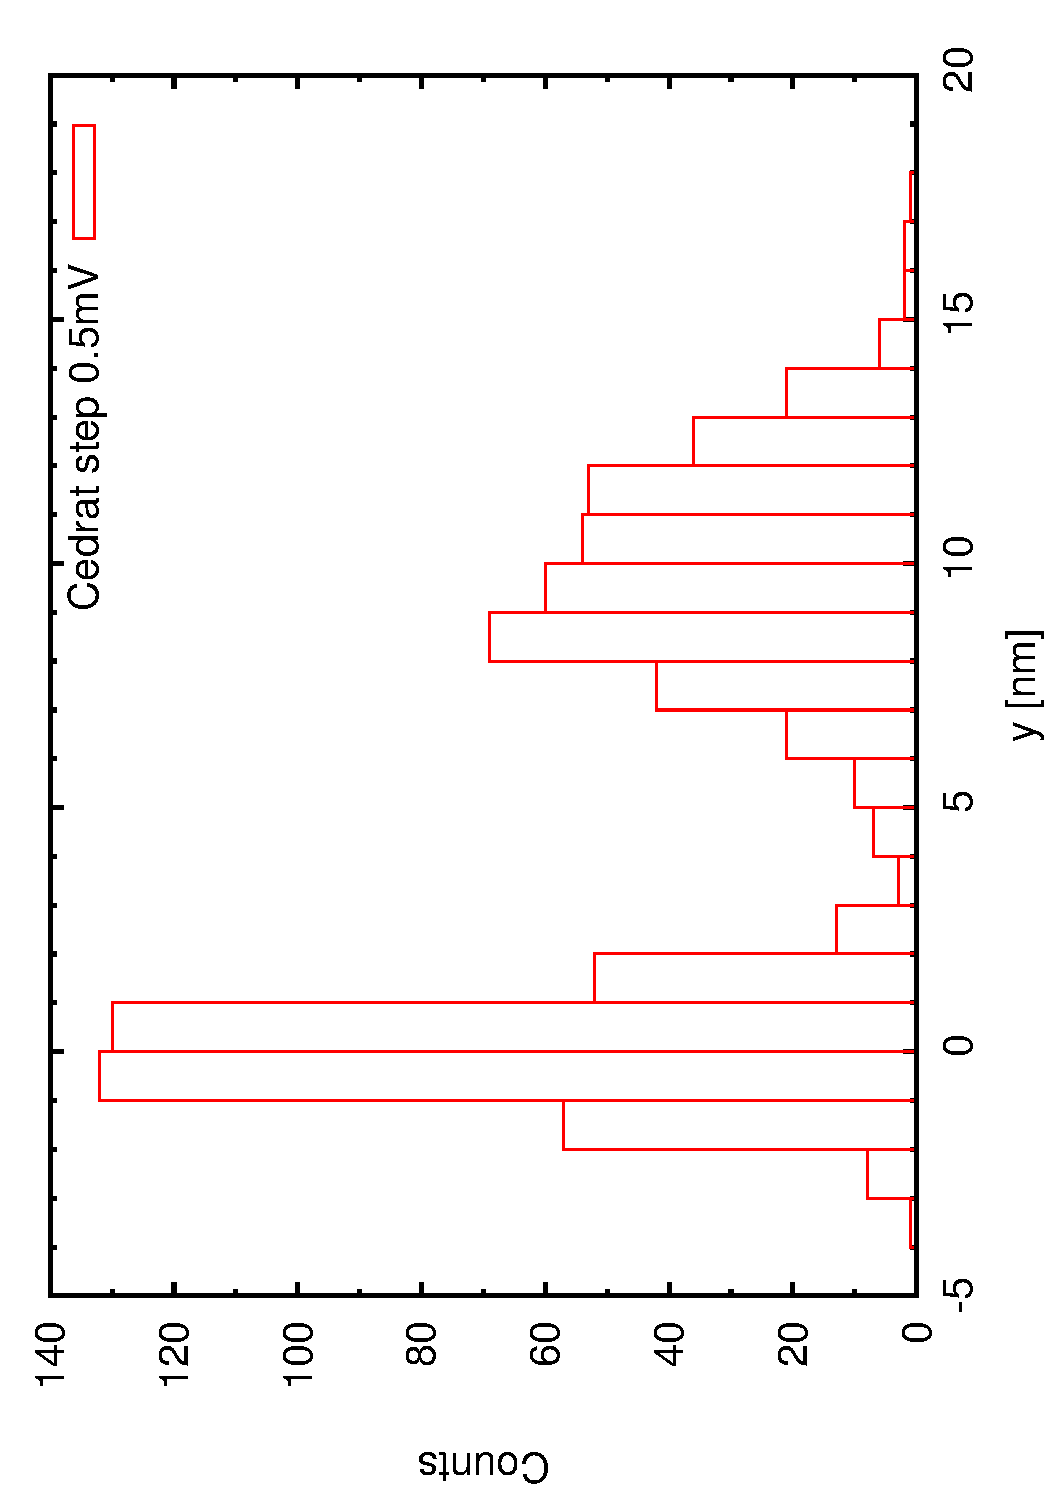
\includegraphics[angle=-90,scale=0.30]{imagestep12a.pdf}\caption{Minimum voltage setting variation back and forth tested was 0.5 mV.}\label{f:Cedratstepstab}
\end{subfigure}\hspace*{1.5cm}
\begin{subfigure}{0.4\textwidth}
 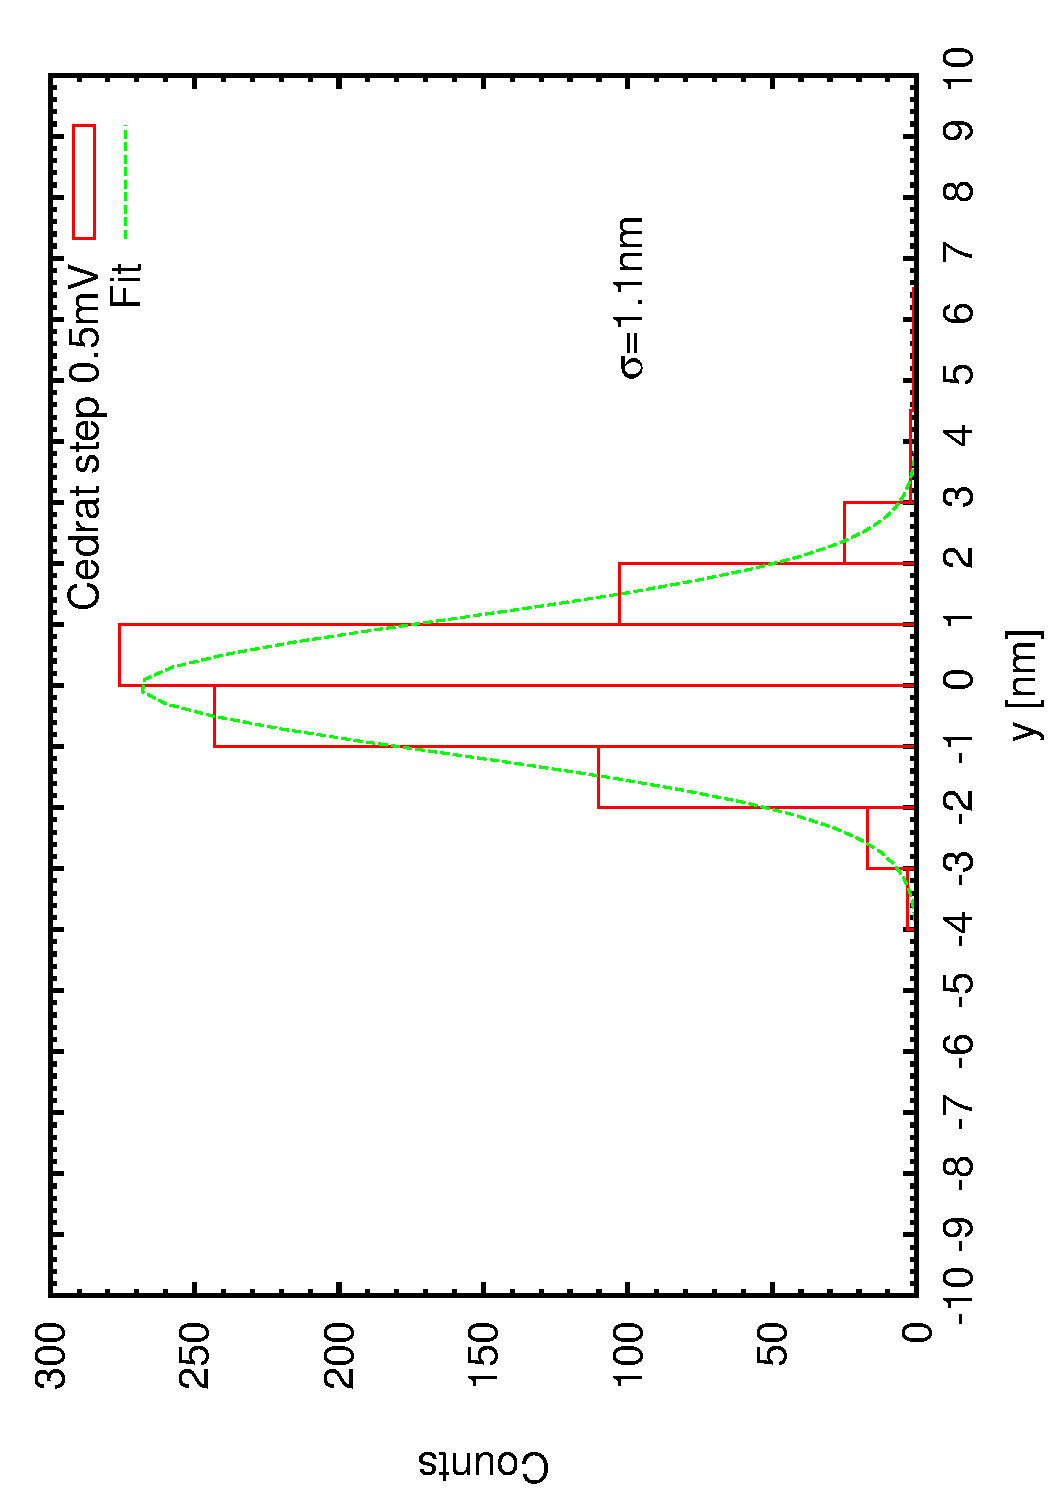
\includegraphics[angle=-90,scale=0.30]{imagestep12.pdf}\caption{Stability at fixed voltage setting.}\label{f:Cedratstab}
\end{subfigure}\caption{Block AB movers minimum step and stability.}\label{f:Cedratstability}
\end{figure}
Coupling effect of horizontal displacement on the vertical plane was also tested. Fig (\ref{f:Cedratcoupling}) shows vertical position variation of 2.5 $\mu$m (1\%) of total horizontal dynamic range.\par
\begin{figure}[!htb]
\centering
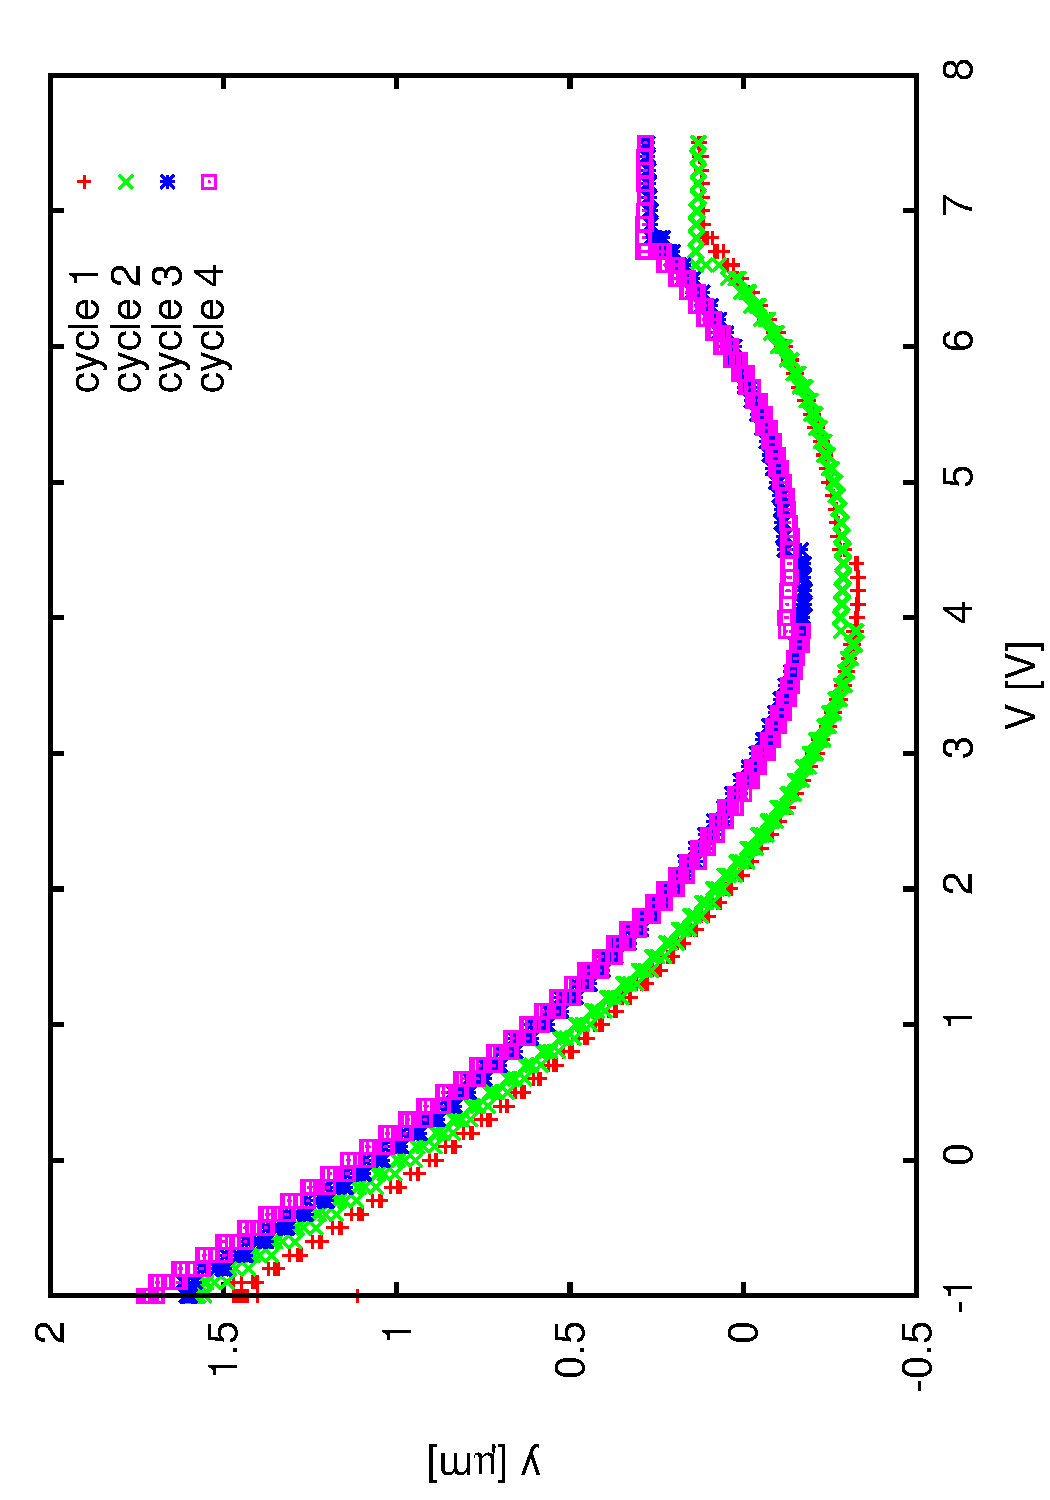
\includegraphics[scale=0.32,angle=-90]{image62.pdf}\caption{Horizontal to vertical movers coupling.}\label{f:Cedratcoupling}
\end{figure}
Only the readbacks from strain gauges are available after installation. Results from readback linearity with respect to voltage setting on ranges below 1 V show that readbacks are limited by electrical noise of $0.8$ mV. This noise is gaussian, and its effect can be minimized by averaging over several readings. This noise does not affect stability because the readbacks and the feedback loop are independent.

\subsubsection{Block C movers, PI}
Linearity was tested in the four cycles with feedback. Fig. (\ref{f:PImsteps}) shows the mover step and Fig. (\ref{f:PIlinres}) shows the residuals from the linear fitting substraction on each cycle.\par
\begin{figure}[!htb]
 \centering\hspace*{-0.6cm}
\begin{subfigure}{0.4\textwidth}
 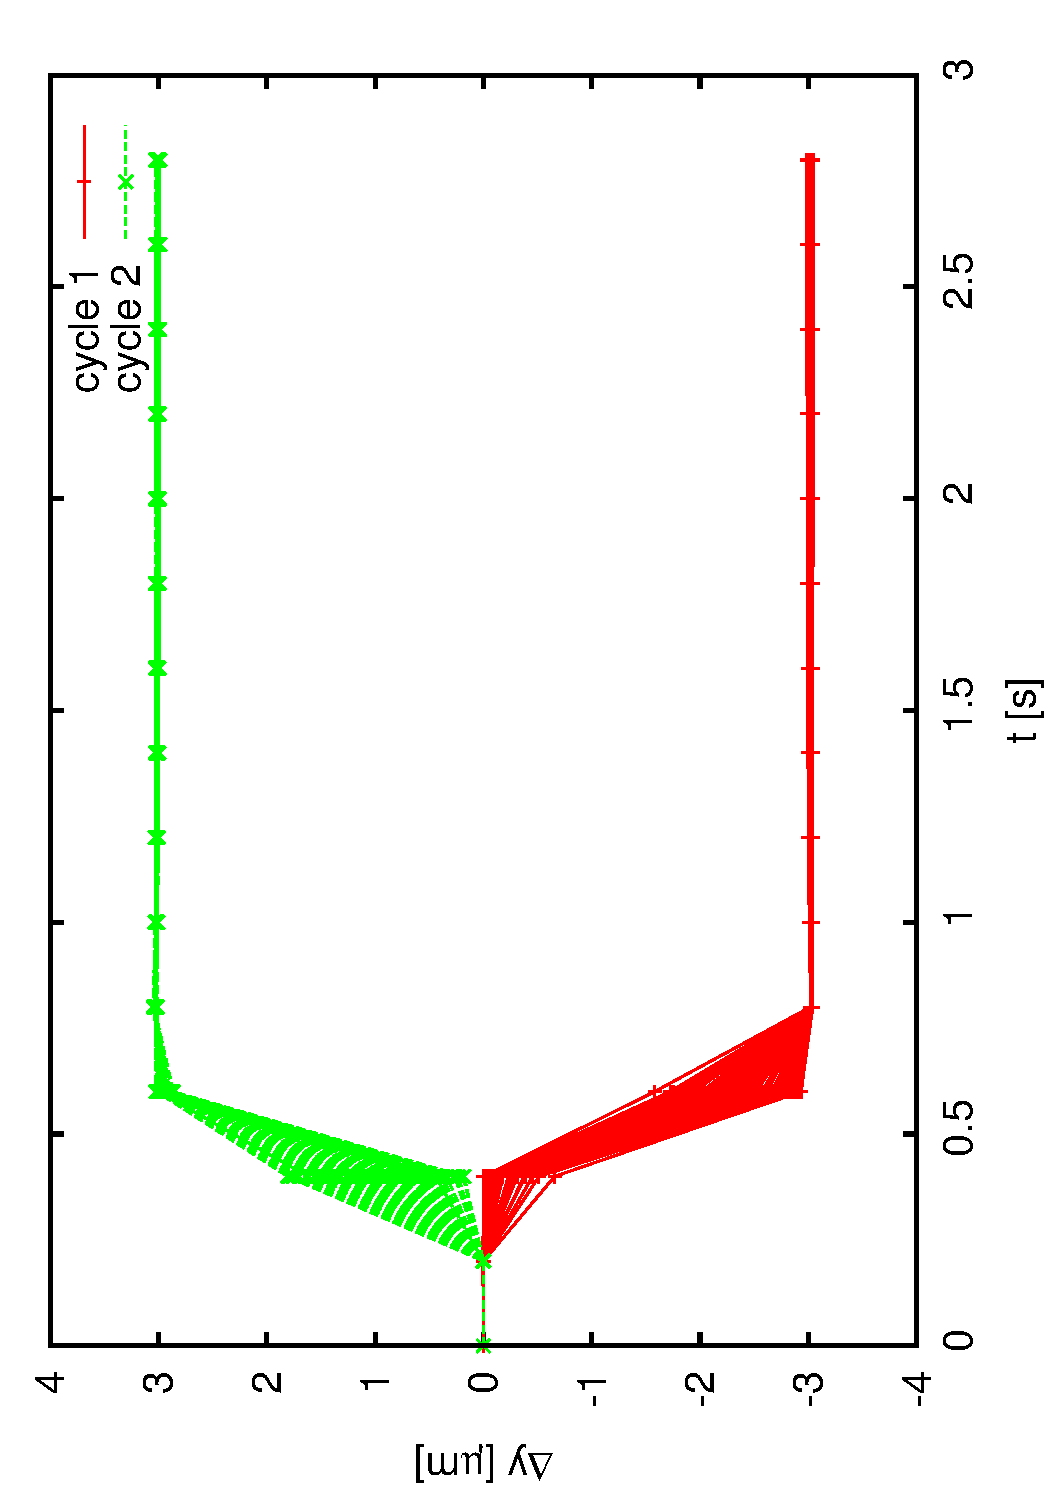
\includegraphics[angle=-90,scale=0.30]{image04.pdf}\caption{Settling speed with feedback for PI movers.}\label{f:PImsteps}
\end{subfigure}\hspace*{1.5cm}
\begin{subfigure}{0.4\textwidth}
 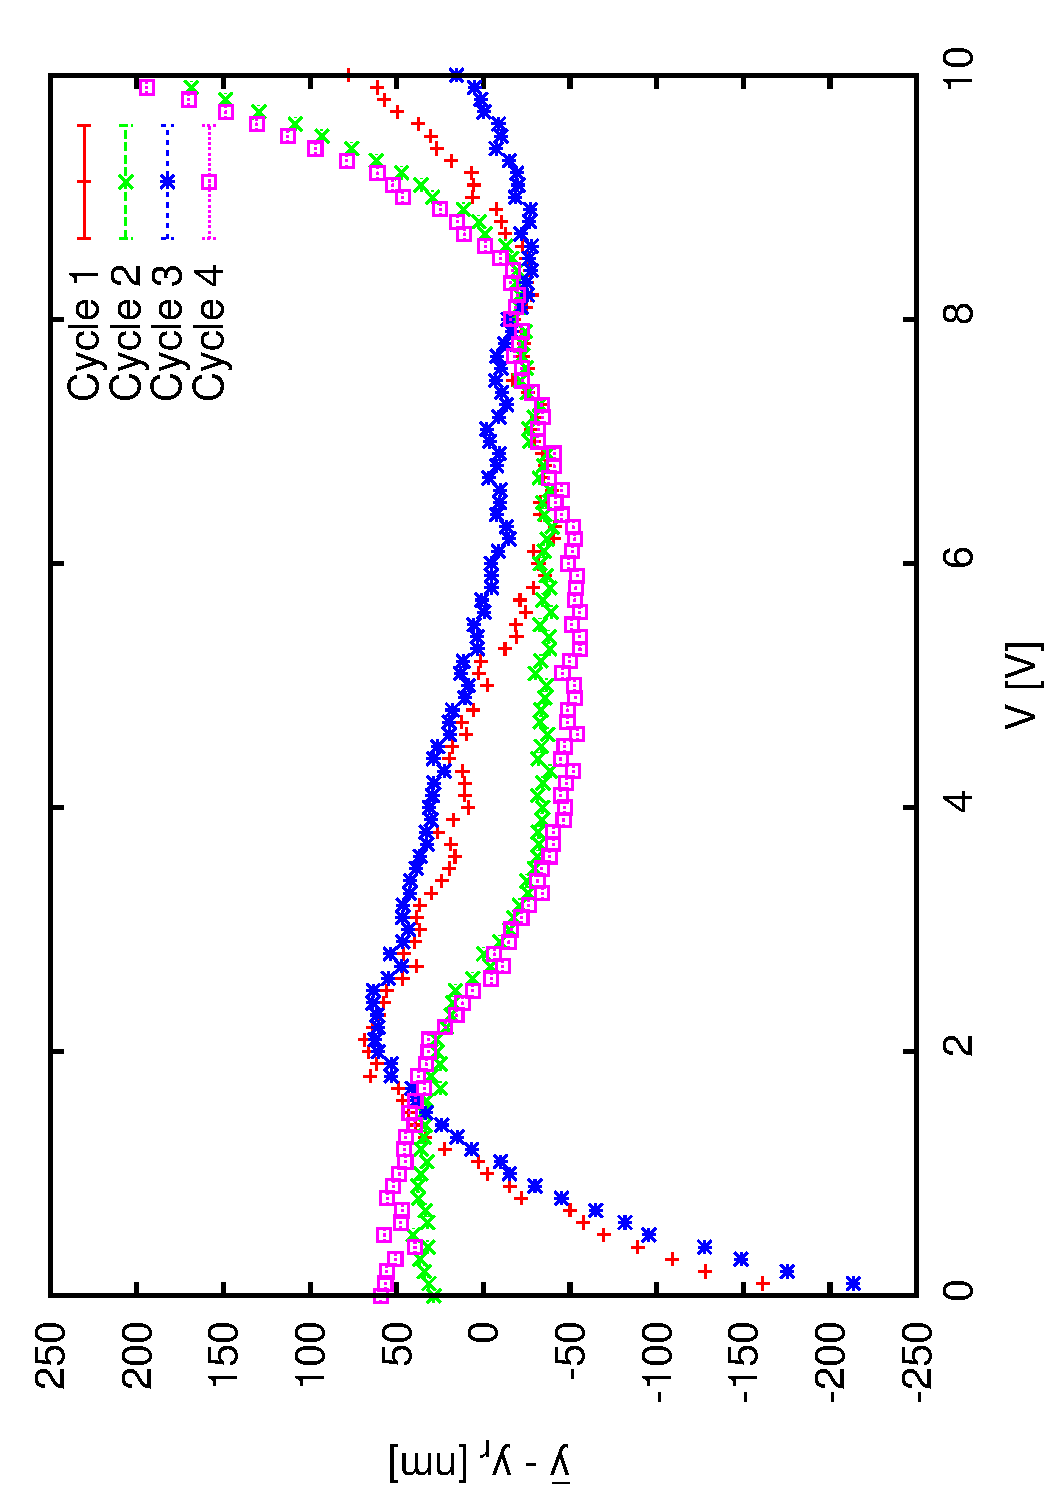
\includegraphics[angle=-90,scale=0.30]{image06e.pdf}\caption{Residual non-linearity (with fb), after substraction of linear fitting on PI movers.}\label{f:PIlinres}
\end{subfigure}\caption{Block C movers, linearity test over four cycles.}\label{f:PIfeedback}
\end{figure}
The calibration mean from these 4 cycles is $C_{mC} = (30.002\pm7)\mu$m/V. This value is valid for ranges were the residual is constant, therefore, it is recommended to use the movers with voltage settings in the middle of the total dynamic range and/or scans over less than 1 V.\par
The step stability was tested by moving back and forth the voltage setting hundreds of times. Fig. (\ref{f:PIstepstab}) shows that 20 nm steps are observable and Fig. (\ref{f:PIstab}) shows 1.13 nm of stability on each setting.\par
\begin{figure}[!htb]
 \centering\hspace*{-0.6cm}
\begin{subfigure}{0.4\textwidth}
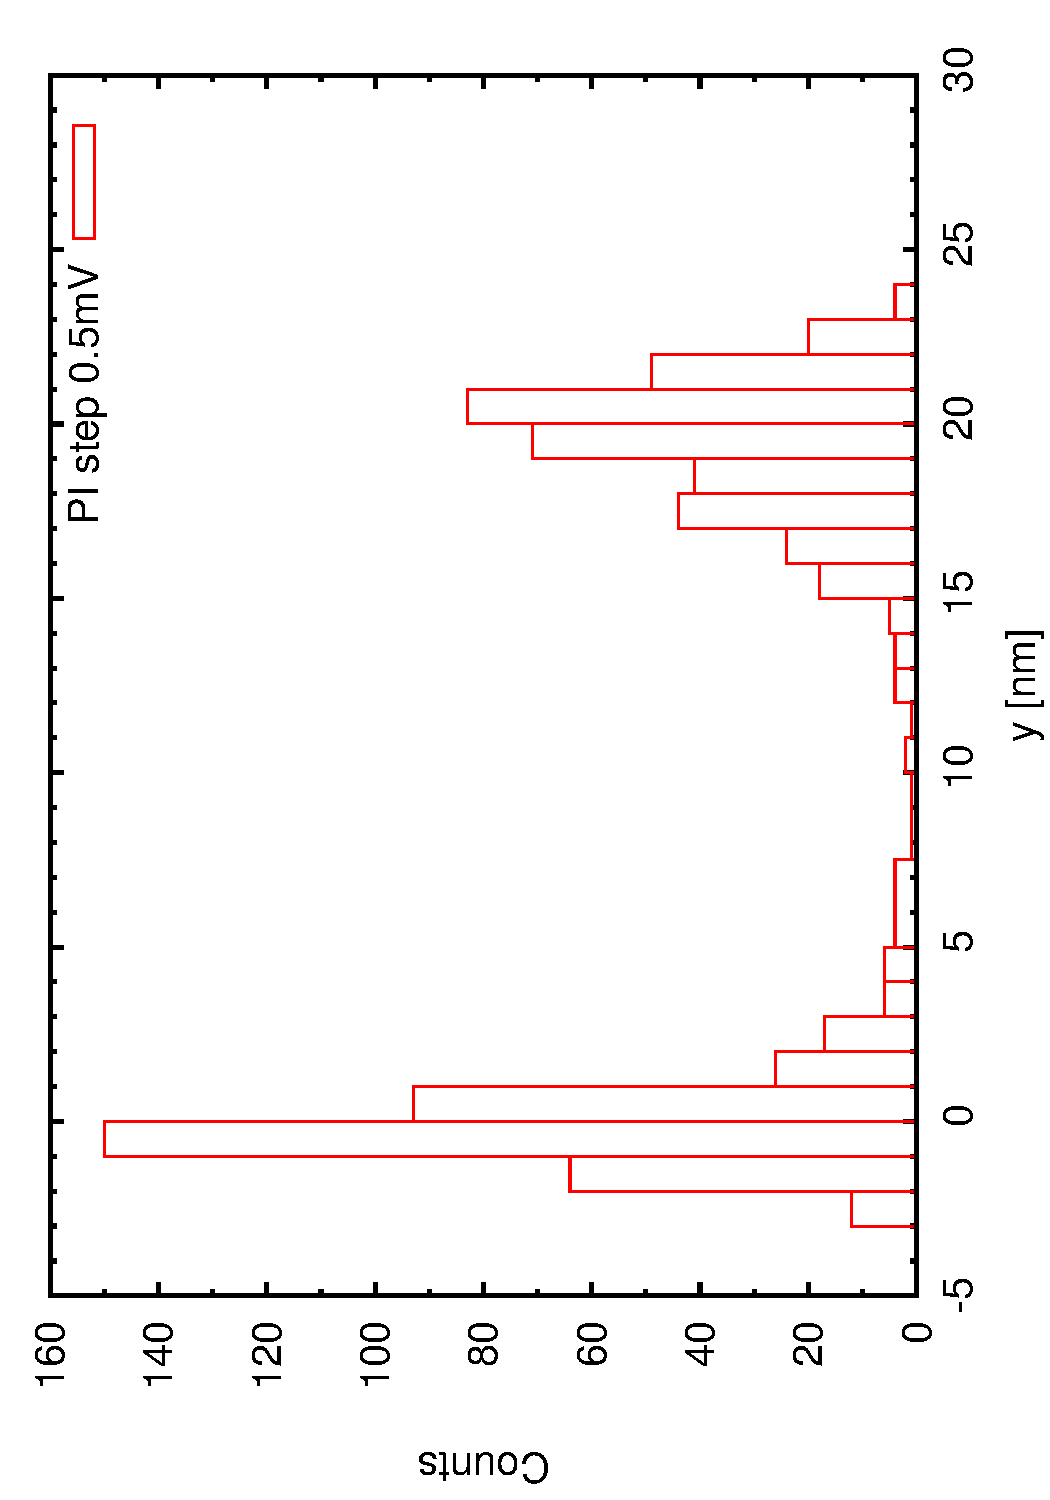
\includegraphics[angle=-90,scale=0.30]{imagestep01a.pdf}\caption{Minimum voltage setting variation back and forth tested was 0.5 mV.}\label{f:PIstepstab}
\end{subfigure}\hspace*{1.5cm}
\begin{subfigure}{0.4\textwidth}
 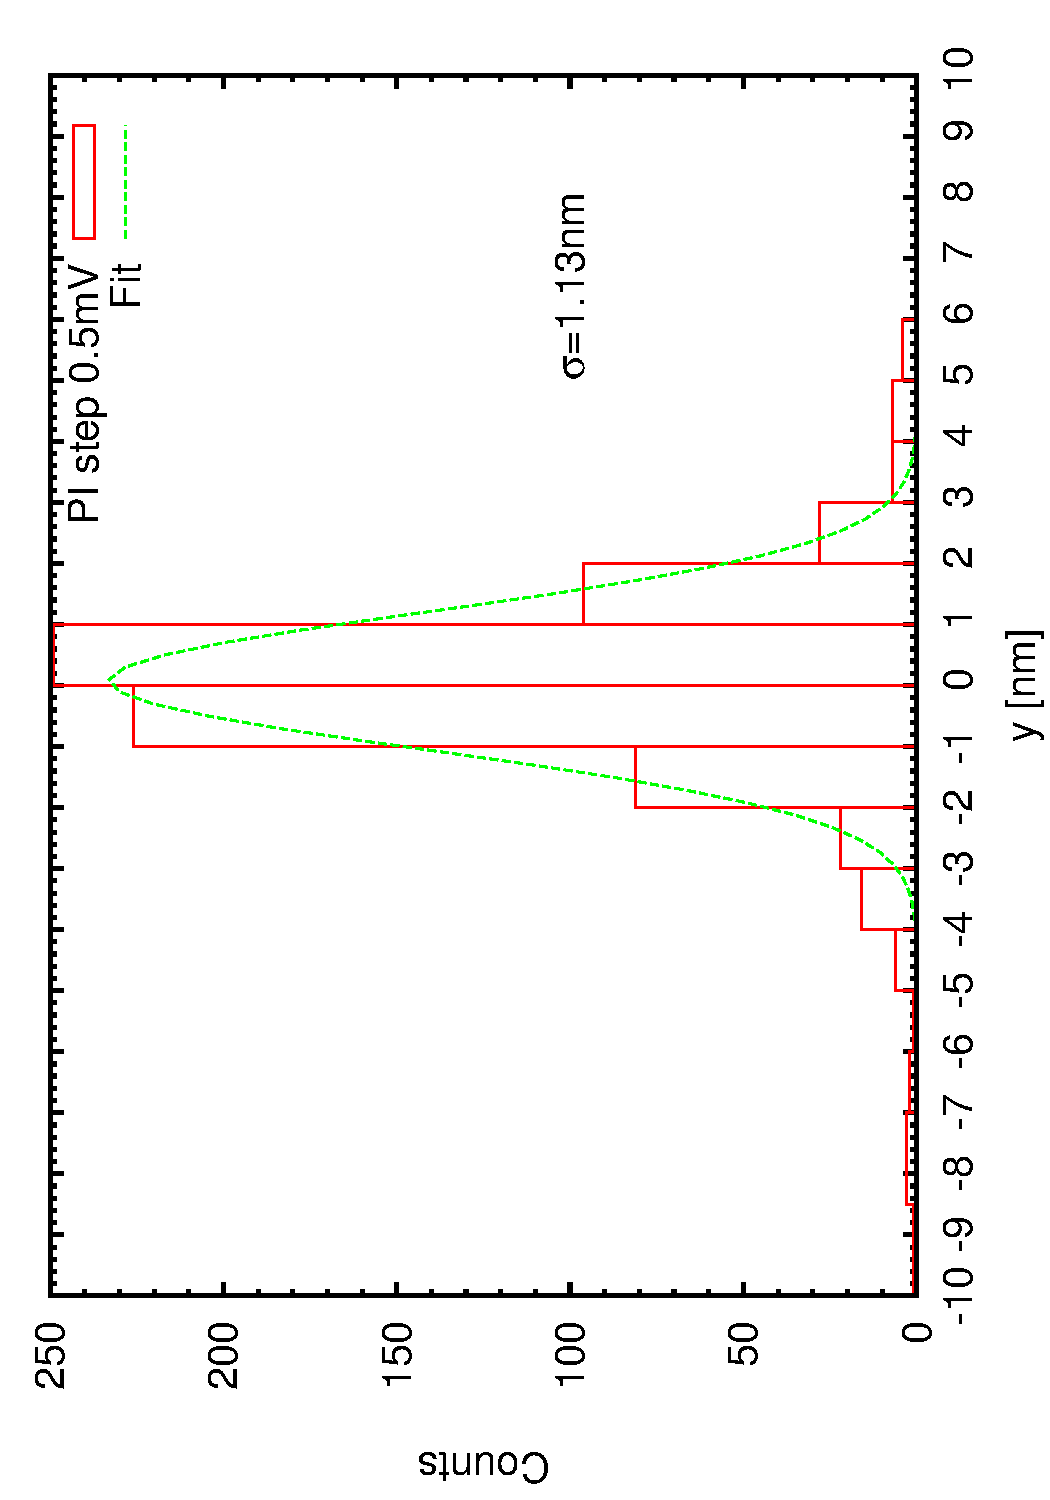
\includegraphics[angle=-90,scale=0.30]{imagestep01.pdf}\caption{Settling speed with feedback for PI movers.}\label{f:PIstab}
\end{subfigure}\caption{Stability at fixed voltage setting.}\label{f:PIstability}
\end{figure}
Coupling effect of horizontal displacement on the vertical plane was also tested. Fig (\ref{f:PIcoupling}) shows vertical position variation of 3 $\mu$m (1\%) of total horizontal dynamic range.\par
\begin{figure}[!htb]
\centering
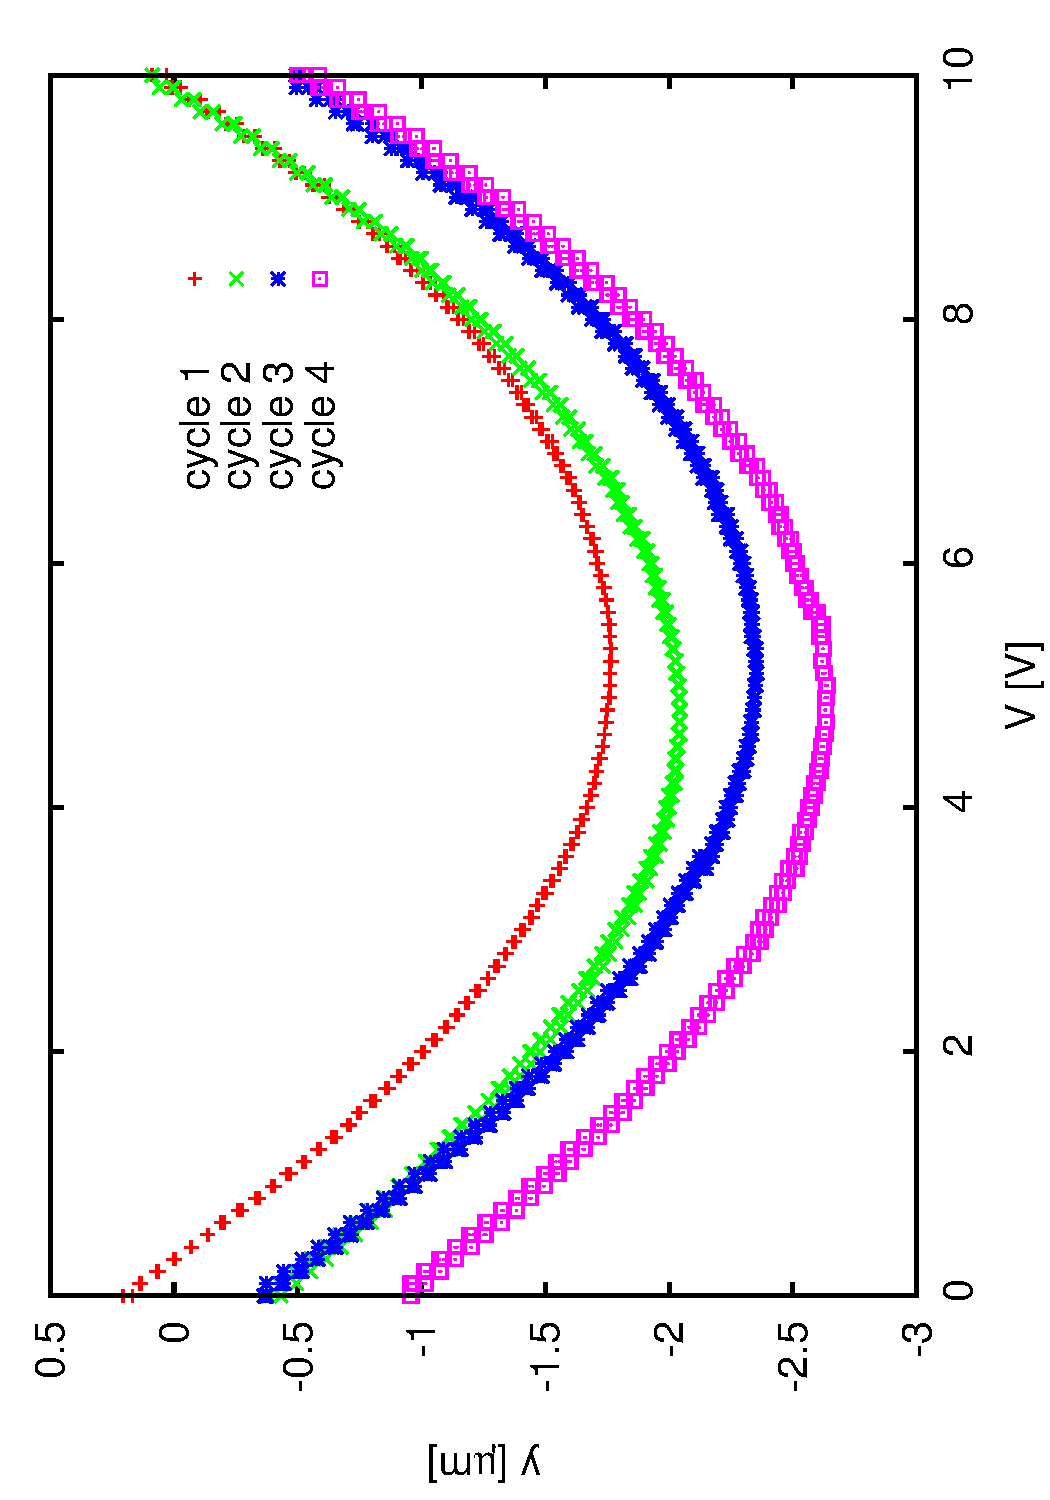
\includegraphics[scale=0.32,angle=-90]{image42.pdf}\caption{Horizontal to vertical movers coupling.}\label{f:PIcoupling}
\end{figure}
Only the readbacks from strain gauges are available after installation. Results from readback linearity with respect to voltage setting on ranges below 1 V show that readbacks are limited by electrical noise of $5.3$ mV. This noise is gaussian, and its effect can be minimized by averaging over several readings. This noise does not affect stability because the readbacks and the feedback loop are independent.

\subsection{Cavity response calibration $C_c$}\label{s:calibration}
During beam time the cavity position is systematically changed and the amplitud of the cavity output signal is measured. Calibration is calculated from the movers voltage readbacks and choosing the signal peak from the acquired waveform,  giving the factor $C_c=I'/V$ [a.u./V], and the IQ rotation angle $\phi$.\par
Input signal can be attenuated from 0 dB to 70 dB in order to keep it inside of the electronics linear response and acquisition system limits. The system response with attenuation change can be seen in Fig. (\ref{f:calatt}) where the variation of calibration is withing $\pm5\%$ for charge between $(0.4\sim0.5)\times10^{10}$ particles, except for IPBy at 0 dB. The reason for this is due to saturation of electronics shown in Section \ref{s:dynrange}.
\begin{figure}[!htb]
 \centering\hspace*{-0.6cm}
 \begin{subfigure}{0.4\textwidth}
  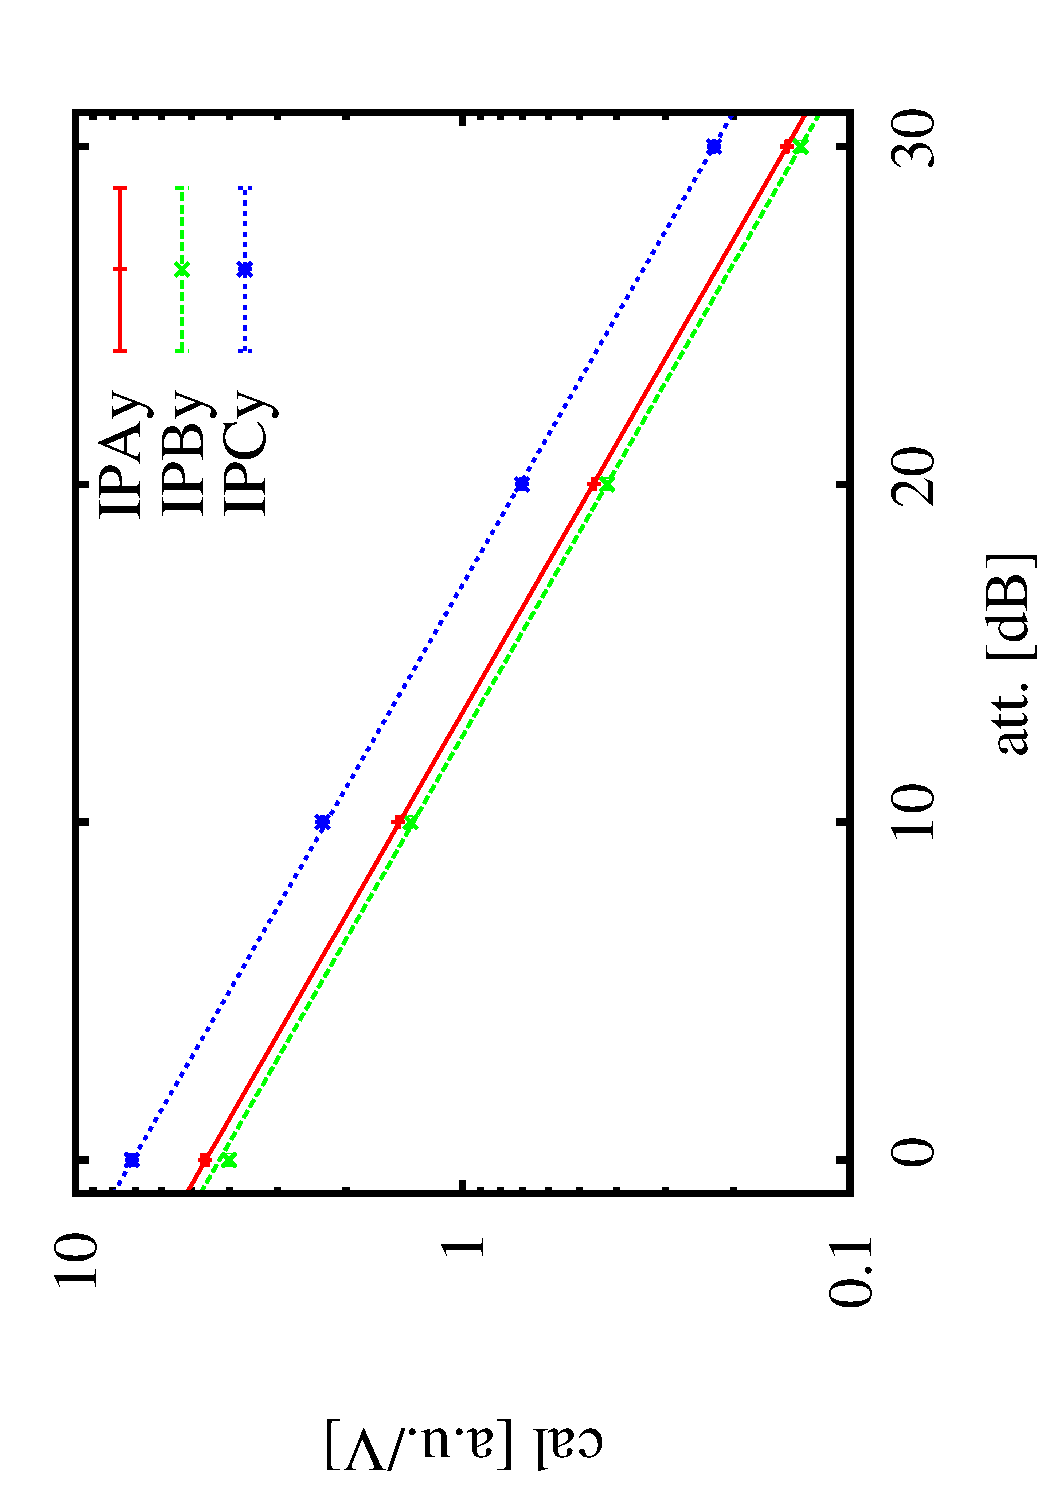
\includegraphics[scale=0.3,angle=-90]{image01_calsy.pdf}\caption{Calibrations in the vertical plane for the three BPMs.}\label{f:calsy}
 \end{subfigure}\hspace*{1cm}
\begin{subfigure}{0.4\textwidth}
  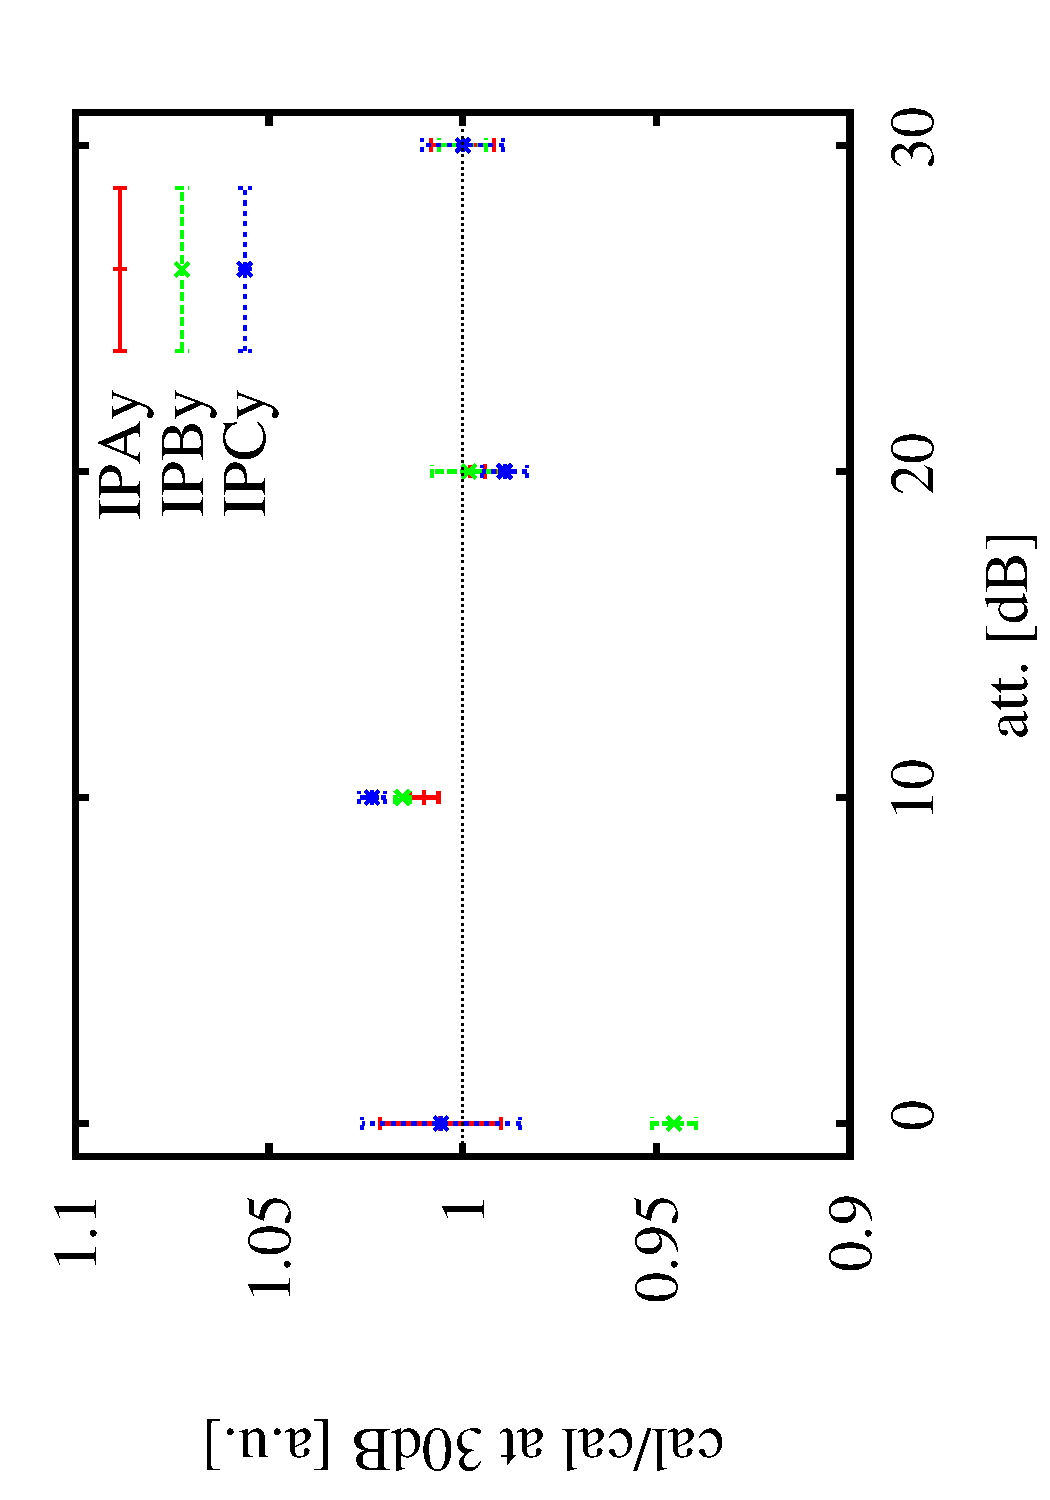
\includegraphics[scale=0.3,angle=-90]{image01_calsynorm.pdf}\caption{Vertical calibrations at 30dB att. is unity and other calibrations are scaled down.}\label{f:calsynorm}
 \end{subfigure}\caption{Calibrations as a function of attenuation.}\label{f:calatt}
\end{figure}

\section{Dynamic Range}\label{s:dynrange}
Dynamic range is measured in this section as the movers voltage range where the cavity response is linear within a tolerance, and therefore it can be translated to position using the movers calibration, $c_m$, in Sect. \ref{s:calcm}. It is limited by the linear response of the cavity sensitivity, the processing electronics and the acquisition system.\par
\subsection{Acquisition System}
Every study case has been performed with signals inside the acquisition system dynamic range, described in \ref{s:acqsys}. The initial FONT board has been recently replaced by a dedicated SIS digitizer with larger and configurable voltage range. This is no longer a limitation.\par
\subsection{Processing electronics and cavity sensitivity}
The processing and cavity response are combined in the calibration study showing linearity above $\pm5\%$ in Sect. \ref{s:calibration}. However, Fig. \ref{f:calsynorm} shows that IPBy calibration is outside this range at 0 dB attenuation. In order to explain this behaviour the $Q'$ signals from calibrations are shown in Fig. \ref{f:Qp}, where it is visible the difference between IPAy and IPCy with respect to IPBy. The decay of IPAy and IPCy $Q'$ signals is consistent with system resolution studies shown in Sect. \ref{s:resolution}. However, IPBy $Q'$ signal is close to ($0.2\sim0.3$)V in the attenuation range from 0 to 20 dB.\par% As the $Q'$ sensitivity derives from the $I'$ sensitivity, it shows that the IPBy signal response is constant along the three attenuation levels.\par
\begin{figure}[!htb]
\centering
 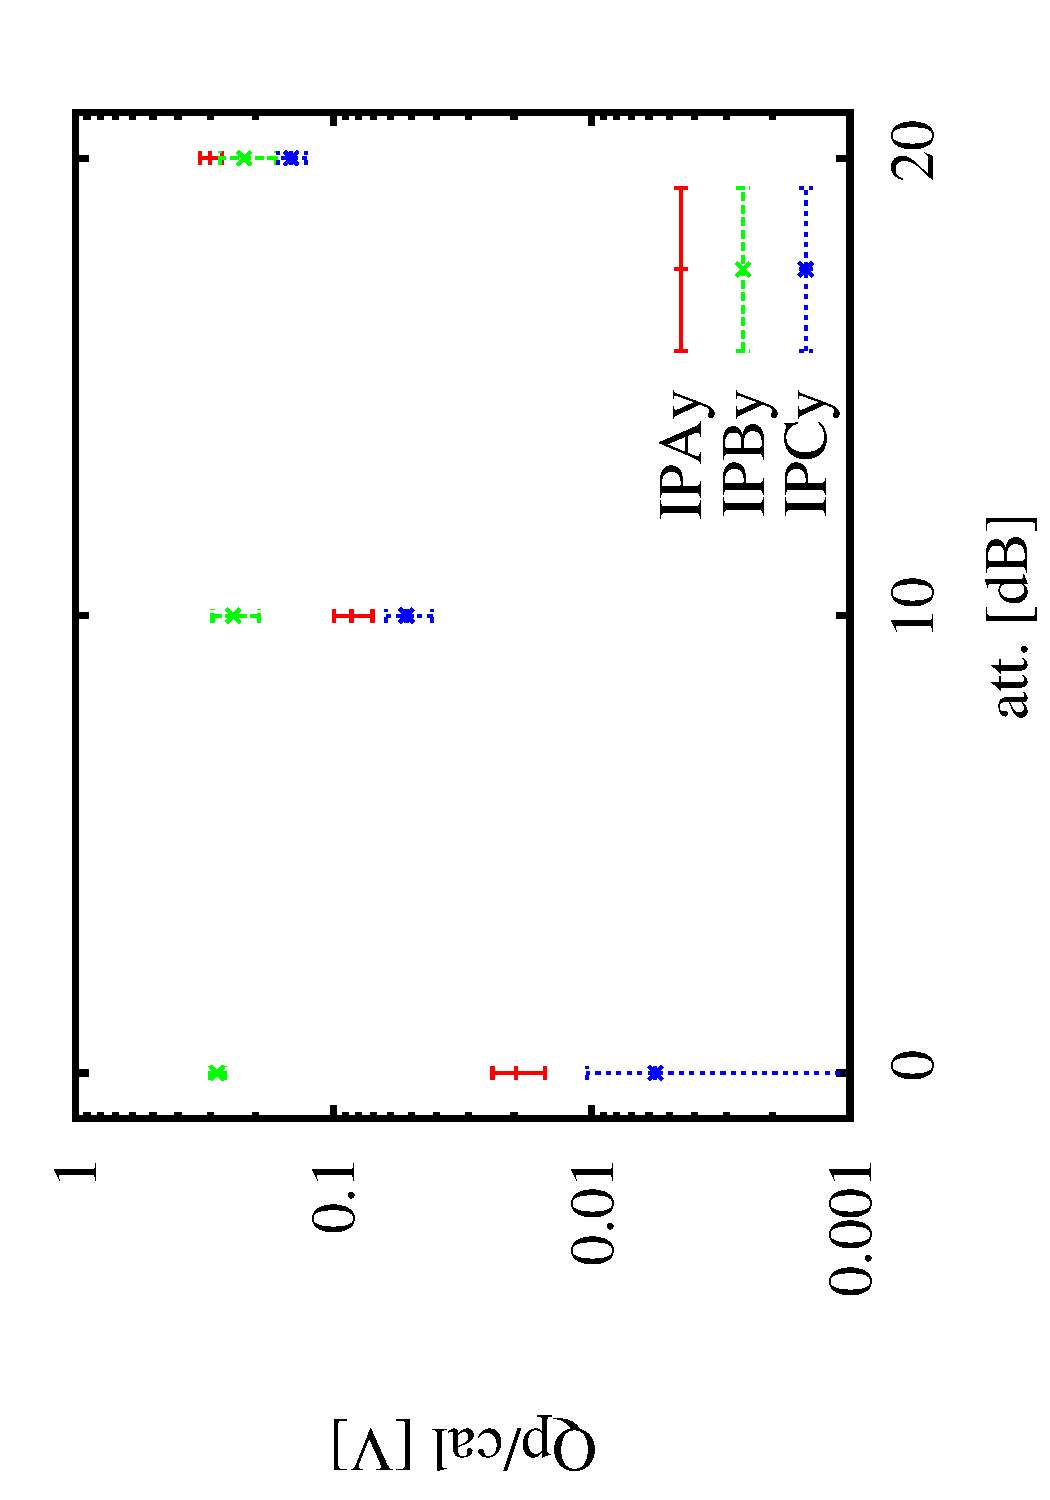
\includegraphics[scale=0.3,angle=-90]{image01_Qp.pdf}\caption{Effect of attenuation in $Q'$ signals from calibrations. Errors bars are RMS.}\label{f:Qp}
\end{figure}
In the same way, the IPBy calibration vs charge is shown in Fig. \ref{f:chargescan}, where the calibration values have been normalized to the minimum charge and attenuation is fixed at 10 dB. The calibration constant decays by more than $5\%$ at charges above $0.4\times10^{10}$ particles.\par
Using the non saturated calibration at $0.36\times10^{10}$ and 10 dB att. we obtain an IPBy dynamic range of 0.36 V, equivalent to 11 $\mu$m using $c_{mAB}$, where cavity calibration $c_B$ varies less than $ \pm5\%$.\par
IPBy $Q'$ signal fills up almost all dynamic range at 10 dB attenuation and $0.4\times10^{10}$ particles, and it is saturating the processing electronics at 0 dB.\par
\begin{figure}[!htb]
\centering%\hspace*{-0.6cm}
% \begin{subfigure}{0.4\textwidth}
 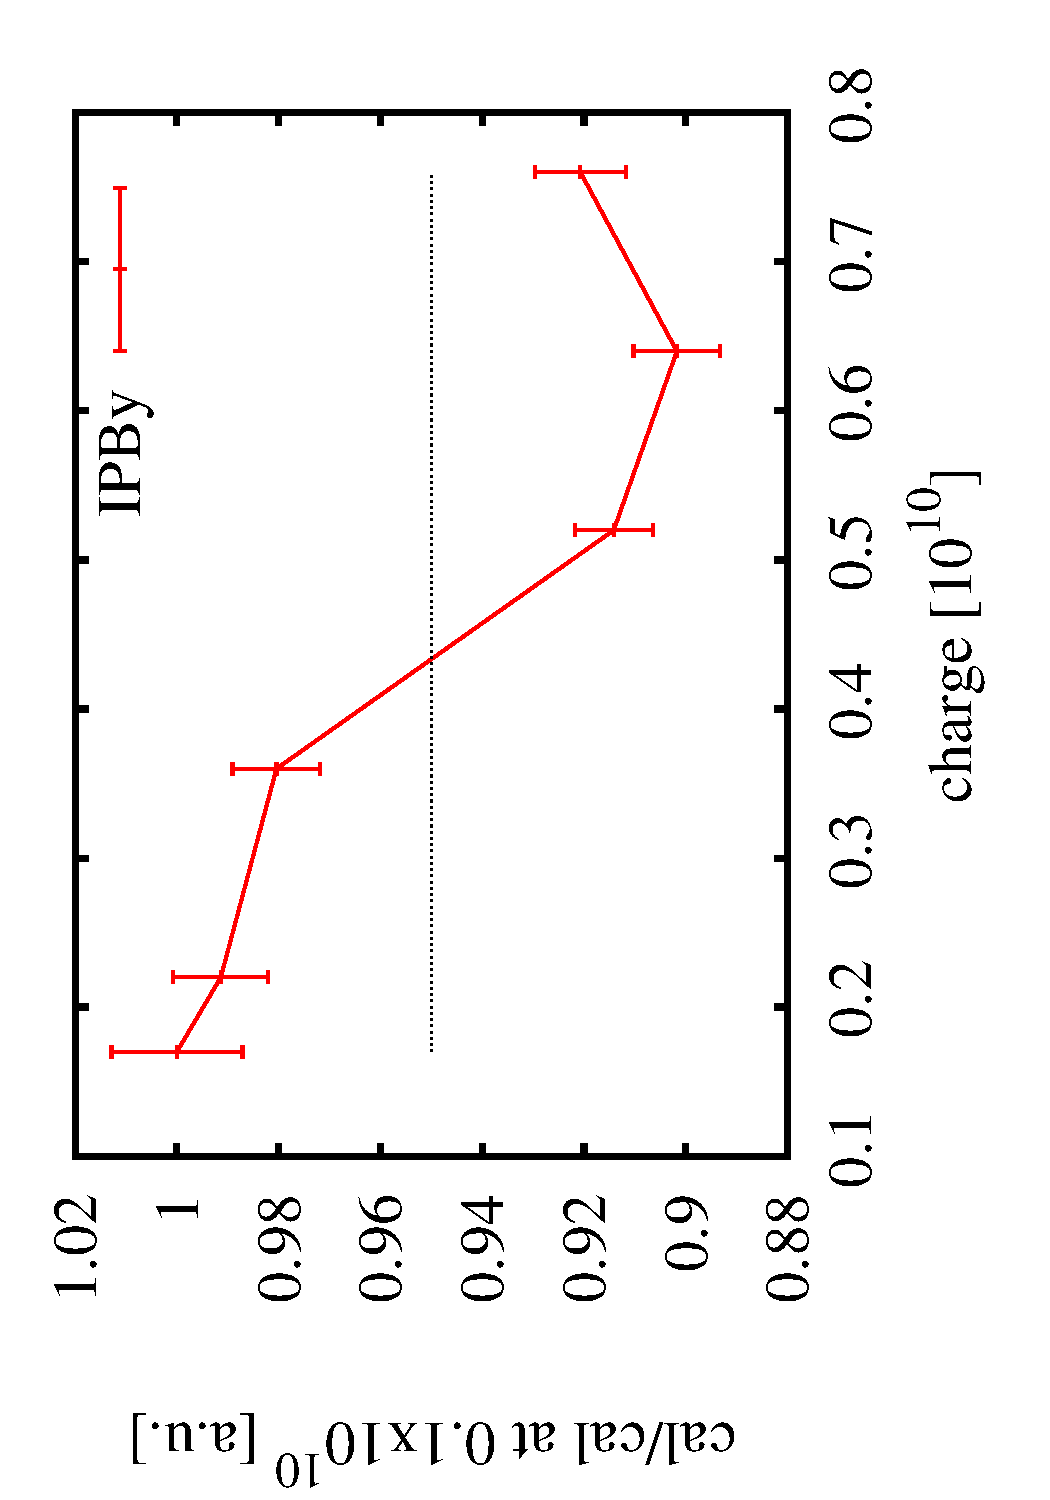
\includegraphics[scale=0.3,angle=-90]{image01_Calvscharge.pdf}\caption{IPBy Calibration vs charge normalized to the calibration at minimum charge.}\label{f:chargescan}
% \end{subfigure}\caption{Cavities $Q'$ signal and calibration charge scan for IPBy normalized to the minimum charge.}
% \hspace*{1cm}\\
% \begin{subfigure}{0.4\textwidth}
%  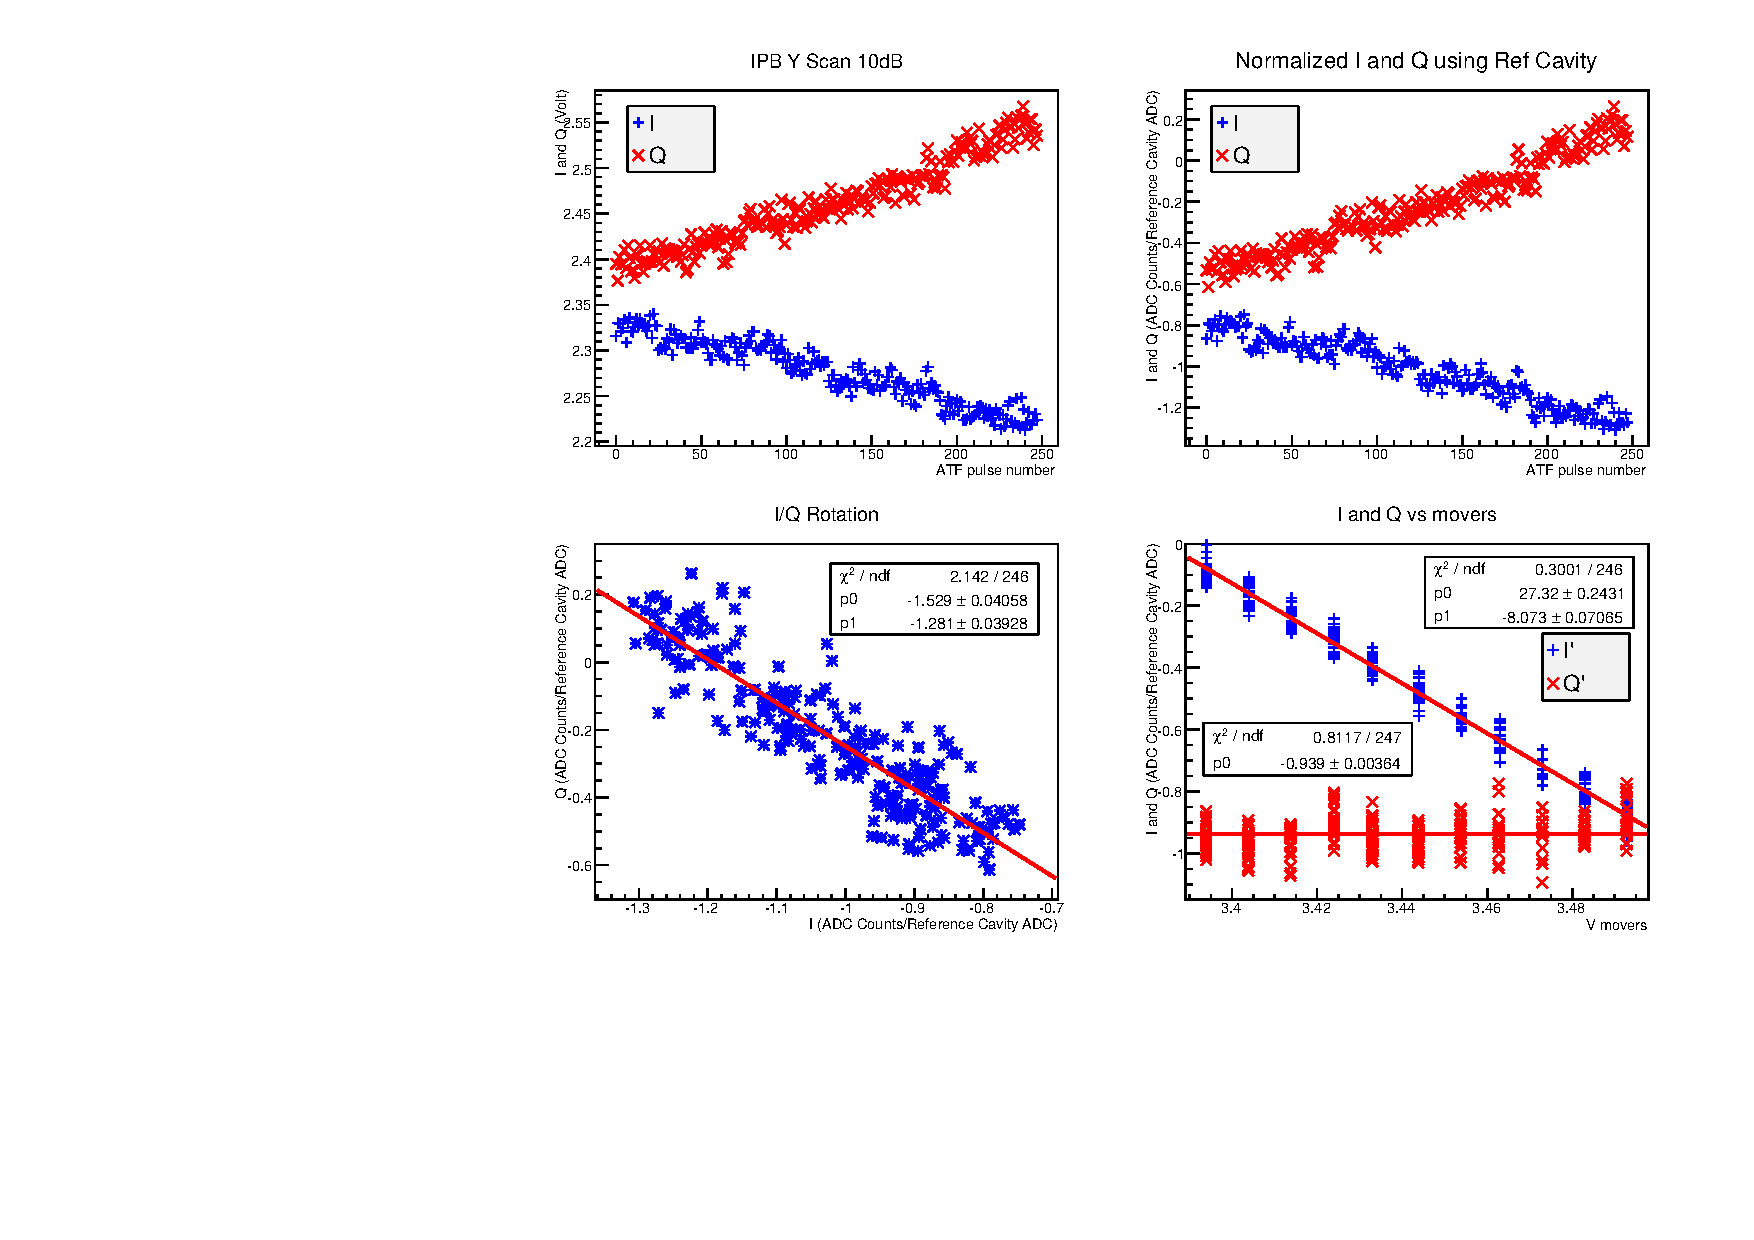
\includegraphics[scale=0.6,angle=0]{IPByCal11_10dB_sample68.pdf}\caption{Calibration at .}\label{f:IPBydynrange}
% \end{subfigure}
\end{figure}
To predict the measured dynamic range of IPBy it is necessary to put extra 6dB of attenuation in the processing electronics gain model (Sect. \ref{s:processing}) . At the moment, it has been attributed to lower than expected sensitivity of the cavities in Section \ref{s:resosensi} and/or cable loss in the processing electronics interconnexion.\par

\section{Resolution}\label{s:resolution}
Resolution is measured in nm using the calibration results from Sect. \ref{s:cals}. It is limited by the cavity sensitivity, the electronics noise floor and the acquisition system resolution.\par
\subsection{Acquisition System}
The acquisition system resolution is specified in Sect. \ref{s:acqsys}. Only the oscilloscopes had lower than required resolution, however, they have already been replaced by a dedicated SIS digitizer. This is no longer a limitation.\par
\subsection{Noise floor and cavity sensitivity}
The BPMs, processing electronics and conexions along the BPM signal path generate noise limiting the minimum detectable waveform. This minimum is estimated by scanning the measured jitter vs the attenuation value.\par
At large attenuations the noise floor is bigger than the BPM signal, while at low attenuations is the opposite. There is an inflection point where both are relevant. The cavity calibration are used to scale it in nm.\par
The jitter acquisition is the measurement of bunch position over several hundreds of pulses with an static BPM position setting. 
The readings from the 3 BPMs are shown in Fig. (\ref{f:resojitter}). Jitter for the three BPMs is in the order of $300\sim400$nm. At 40 dB the limit imposes over the signal and by extrapolation the resolution limit per BPM is 10 nm for IPAy and IPBy, and 20 nm for IPCy at 0 dB.\par
\begin{figure}[!htb]
\centering\hspace*{-0.6cm}
\begin{subfigure}{0.4\textwidth}
 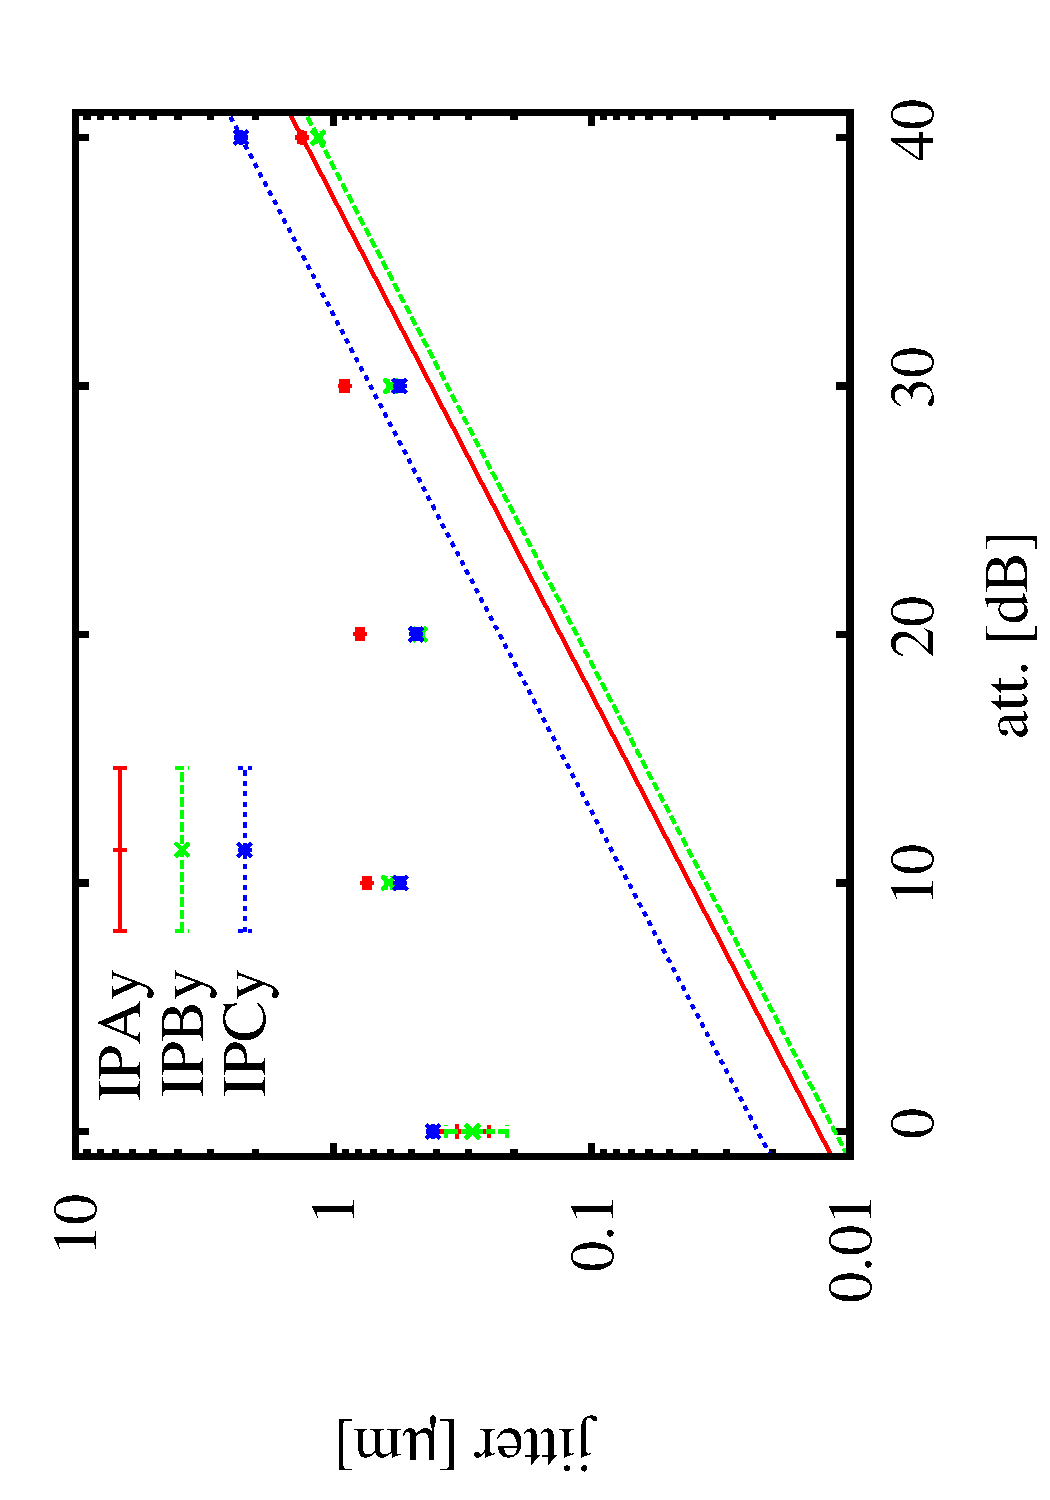
\includegraphics[scale=0.3,angle=-90]{image01_jitter.pdf}\caption{Jitter measurement for the 3 BPMs.}\label{f:resojitter}
\end{subfigure}\hspace*{1cm}
\begin{subfigure}{0.4\textwidth}
 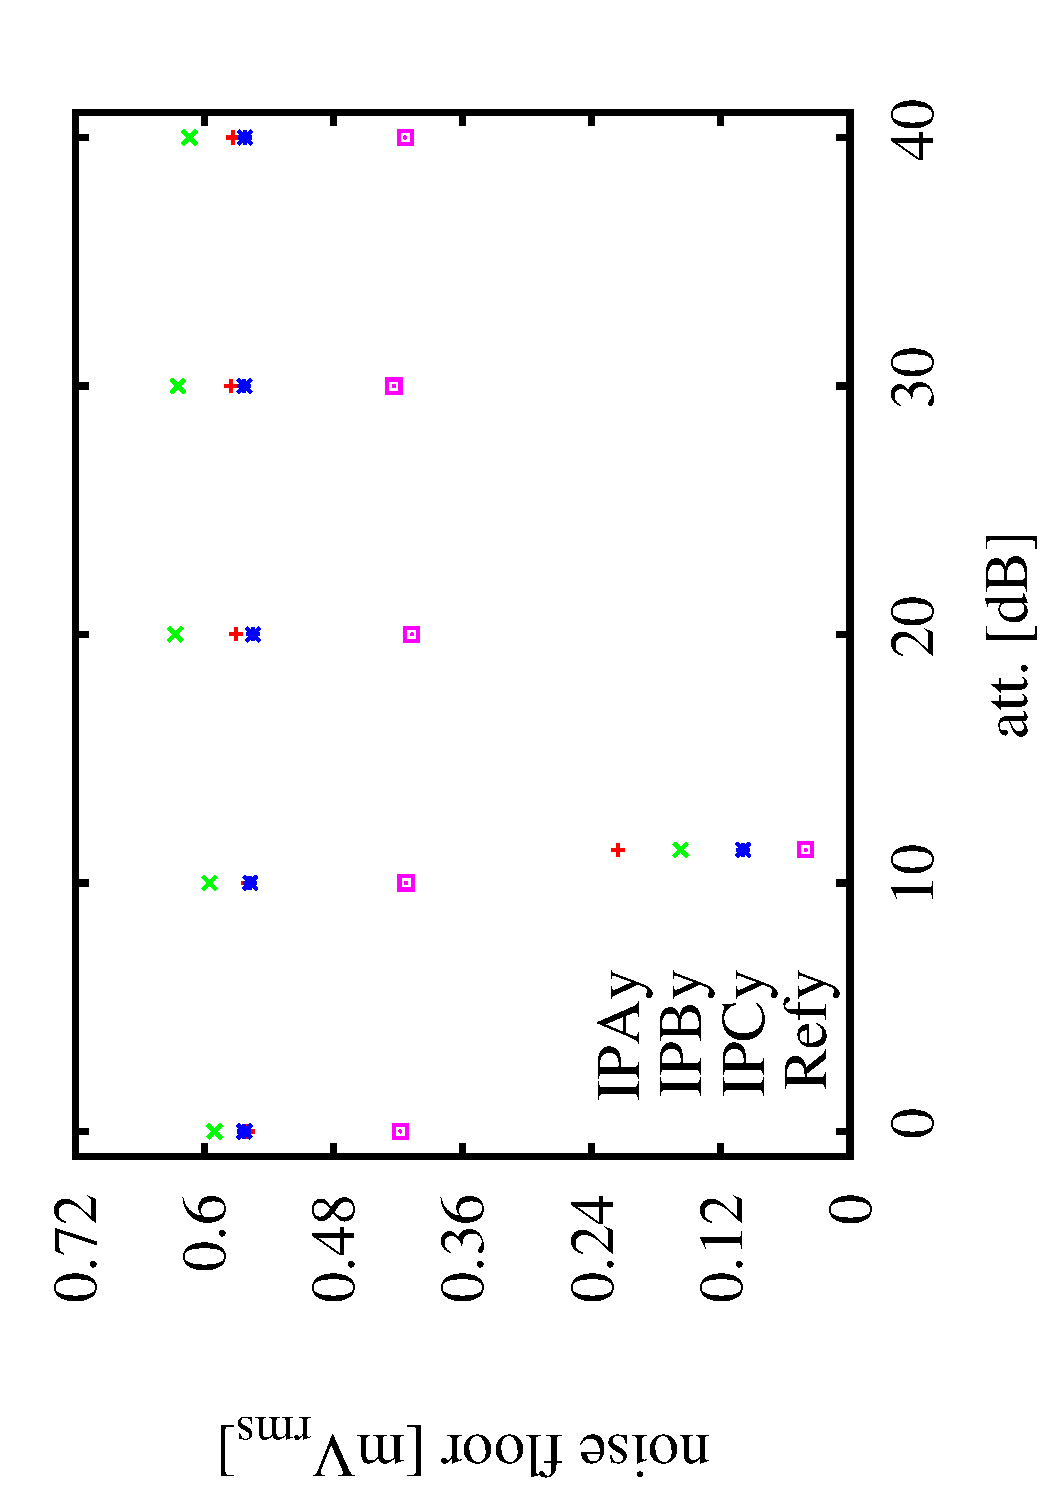
\includegraphics[scale=0.3,angle=-90]{image01_noisetot.pdf}\caption{Noise per channel for the 3 BPMs.}\label{f:resonoisetot}
\end{subfigure}\caption{Resolution extrapolation by jitter measurement for the 3BPMs.}\label{f:resojitternoise}
\end{figure}
It is also clear that IPC shows worst resolution limit that IPA and IPB. Two possibilities arise: the electronics noise is larger for IPC or the sensitivity is lower.\par 
\subsubsection{Noise floor}
Fig. (\ref{f:resonoisetot}) shows the noise from the jitter acquisition. It is clear that noise is consistent through out the calibration scan and therefore the difference in jitter seen for IPCy at 40dB att. comes from the calibration factor. Using the total gain to \par
Compatible with \cite{PhysRevSTAB.11.062801}


\subsubsection{Cavity sensitivity}\label{s:resosensi}
Cavity sensitivity and processing electronics gain change the calibration factor. Due to the 6dB mismatch between the mesured dynamic range measured and predicted for IPBy, as shown in Sect. \ref{s:dynrange}, and the lack of charge scans for IPAy and IPCy, it is not possible to conclude about the total gain without making assumptions.\par
However, the signal decay time from waveforms gives information about the cavity sensitivity. 


\section{Status and Conclusions}
Table (\ref{t:IPBPMsStatus}) show summary of the current IP-BPMs results
\begin{table}[hbt]
\centering
\begin{tabular}{l|l|l|p{4cm}}\hline
PARAMETER & REQUIREMENT & STATUS & Comments\\\hline\hline
Resolution & $\sim$nm & <50nm & Calibration factors ?\newline BPM sensitivity ?\newline Electronics ? \newline X to Y coupling ?\\\hline
Dynamic Range & $\sim$10$\mu$m + extra & $1\mu$m$\sim3\mu$m at 0db & Linear Response of the Cavity ?\newline Electronics ?\newline No extra for alignment + Q' signal \\\hline
Compatibility & IPBSM, EPICS & In work &Calibration Software OK\newline Jitter analysis Software OK\newline IP-BSM, needs common setup \newline EPICs, data still requires off-line analysis\\\hline
Feedback & Operative & Tested	& \\\hline
\end{tabular}\caption{IPBPMs status.}\label{t:IPBPMsStatus}
\end{table}